\documentclass[]{article}
\usepackage{amsmath}		% For generic math symbols
\usepackage{amssymb}		% For mathbb
\usepackage{enumerate}		% For lists indexed by letters
\usepackage{bm}				% For bold letters
\usepackage{enumitem}		% So we can resume counting problem numbers after
% interrupting with text
\usepackage{hyperref}		% For clickable URL links
\usepackage{mathtools}

\setlength{\parindent}{0pt}	% Turns off indentation


% Set some useful commands
\newcommand{\half}{\frac{1}{2}}
\newcommand{\R}{\mathbb{R}}
\newcommand{\C}{\mathbb{C}}
\newcommand{\bbm}{\begin{bmatrix}}
\newcommand{\ebm}{\end{bmatrix}}
\newcommand{\x}{\bm{x}}
\newcommand{\y}{\bm{y}}
\newcommand{\vspan}{\mathrm{span}}
\newcommand{\defeq}{\vcentcolon=}

% Place this command after each problem, before solution (examples below)
\newcommand{\solution}{\vskip 0.5cm \textbf{\large Solution:} \\}

\title{AMATH 352: Problem Set 2}
\author{Dave Moore, dmmfix@uw.edu}

\begin{document}

\maketitle
    {\Large \textbf{Due: Friday January 20, 2017}}

    \section*{Norms:}
    \begin{enumerate}
	\item Find and sketch the closed unit ball in $\R^2$ for the infinity norm. Justify your drawing (your answer for this problem should be more than just a drawing).

	  \solution
      
	  The closed unit ball in $\R^2$ under $\|\cdot\|_{\infty}$
      in $\R^2$ is the set of points that satisfy $\|\bm{x}\|_{\infty}
      \leq 1$. Since $\|\bm{x}\|_{\infty} \defeq max(|x_i|)$, a vector is
      in this set iff
      \begin{gather*}
        -1 \leq x_1 \geq 1 \\
        -1 \leq x_2 \geq 1
      \end{gather*}
      This is just a square with sides of length 2 centered at the origin.
      \begin{center}
        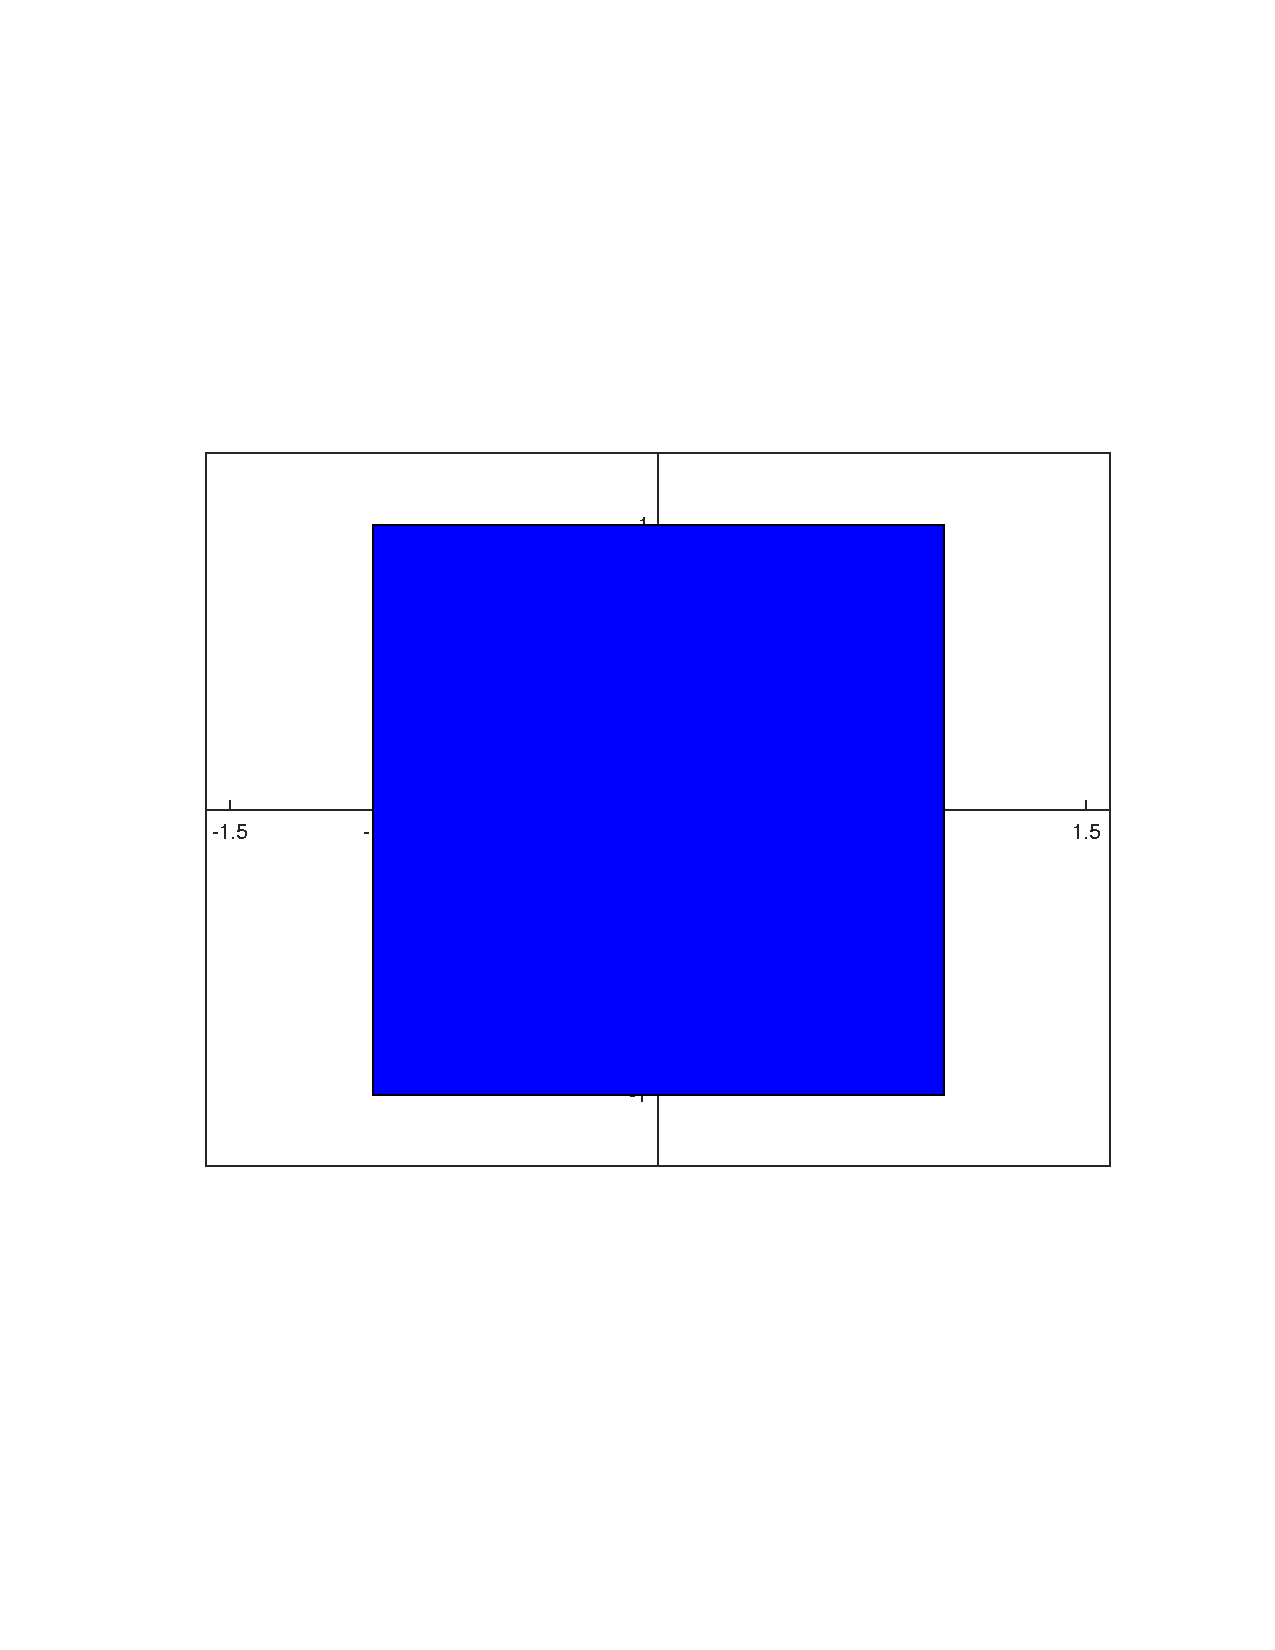
\includegraphics[scale=0.5]{unit_sphere_supnorm.pdf}
      \end{center}
    \end{enumerate}

    \section*{Real Linear Spaces:}

    \begin{enumerate}[resume]
	\item Verify that $\mathbb{C}^2$ (the set of column vectors with two entries which are both in $\mathbb{C}$) is a real linear space, i.e. show that it satisfies the 10 defining properties of a real linear space.

	  \solution
      \begin{enumerate}
      \item $\forall a,b \in \C^2$
        \[
        a + b = \bbm a_1 \\ a_2 \ebm + \bbm b_1 \\ b_2 \ebm = \bbm a_1 + b_1 \\ a_2 + b_2 \ebm
        \]
        Because the complex numbers are closed under addition, each
        $a_i + b_i$ term is also a complex number. The resulting
        vector has 2 elements, and is in $\C^2$, so $\C^2$ is closed
        under addition.
      \item Addition in $\C^2$ is commutative because the complex
        numbers are commutative under addition:
        \[
        a + b = = \bbm a_1 + b_1 \\ a_2 + b_2 \ebm = \bbm b_1 + a_1 \\ b_2 + a_2 \ebm = b + a
        \]
      \item Addition in $\C^2$ is associative because the complex
        numbers are associative:
        \[
        a + (b + c) = \bbm a_1 + (b_1 + c_1) \\ a_2 + (b_2 + c_2) \ebm = \bbm (a_1 + b_1) + c_1 \\ (a_2 + b_2) + c_2 \ebm = (a + b) + c
        \]
      \item The zero vector in $\C^2$ is $\bbm 0 \\ 0 \ebm$:
        \[
        a + \bm{0} = \bbm a_1 + 0 \\ a_2 + 0 \ebm  = \bbm a_1 \\ a_2 \ebm = a
        \]
      \item Because every element $x \in \C$ has an additive inverse
        $-x \in \C$, every element of $\C^2$ also has an additive
        inverse:
        \[
        a + -a = \bbm a_1 + -a_1 \\ a_2 + -a_2 \ebm = \bbm 0 \\ 0 \ebm = \bm{0}
        \]
      \item $\forall x \in \R, z \in \C, xz \in \C$, so $\C^2$ is similarly
        closed under scalar multiplication
        \begin{gather}
          x \in \R, a \in \C^2 \\
          x a = \bbm x a_1 \\ x a_2 \ebm
        \end{gather}
        The $x a_i$ terms are complex numbers, so this 2-element vector is in $\C^2$.
      \item $\forall a,b \in \R, x \in \C^2$
        \[
        (a + b)x = \bbm (a + b)x_1 \\ (a + b)x_1 \ebm  = \bbm a x_1 + b x_1 \\ ax_2 + bx_2 \ebm = ax + b x
        \]
      \item $\forall a \in \R, u,v \in \C^2$
        \[
        a ( u + v ) = a \bbm (u_1 + v_1) \\ (u_2 + v_2) \ebm = \bbm a (u_1 + v_1) \\ a (u_2 + v_2) \ebm = \bbm au_1 + av_1 \\ au_2 + av_2 \ebm = au + av
        \]
      \item $\forall x \in \C^2$
        \[
        1 x = \bbm 1 x_1 \\ 1 x_2 \ebm = \bbm x_1 \\ x_2 \ebm = x
        \]
        $\C^2$ therefore satsifies all ten requirements of a real linear space.
      \end{enumerate}
      
	\item Which of the following sets $W$ are subspaces of $V$ (and hence are linear spaces themselves)? Justify your answers with arguments showing they are closed under addition and scalar multiplication or counterexamples showing they are not.
	  \begin{enumerate}
	  \item $V = \R^4$ and $W = \left\{ \x=\bbm x_1\\x_2\\x_3\\x_4 \ebm\in\R^4: x_1+2x_2 = 0 ~\mathrm{and}~ x_3-x_4=0 \right\}$
	  \item $V=C^0(\R,\R)$ and $W = \{ f\in V : f(3) = 2\}$
	  \item $V = \mathcal{F}(\R,\R)$ and $W$ is the set of all periodic functions of period 1, i.e. the set of all functions $f$ such that $f(x+1)=f(x)$ for all $x\in\R$.
	  \end{enumerate}

	  \solution

	  \begin{enumerate}
	  \item This set is closed under addition and scalar
        multiplication, and is therefore a subspace of $\R^4$. To show
        that the set is closed under addition, we want to show that
        $\forall x,y \in W, z = (x + y) \in W$.
        \[
        z = (x + y) = \bbm x_1 + y_1 \\ x_2 + y_2 \\ x_3 + y_2 \\ x_4 + y_4 \ebm
        \]
        We can see that
        \[\begin{split}
        z_1 + 2z_2 &= (x_1 + y_1) + 2(x_2 + y_2) \\
        &= (x_1 + 2x_2) + (y_1 + 2y_2) \\
        &= 0
        \end{split}\]
        and
        \[\begin{split}
        z_3 - z_4 &= (x_3 + y_3) - (x_4 + y_4) \\
        &= (x_3 - x_4) + (y_3 - y_4) \\
        &= 0
        \end{split}\]
        To show that it is closed under scalar multiplication, need to
        show that $\forall \alpha \in \R, x \in W$
        \[
        \alpha x = \bbm \alpha x_1 \\ \alpha x_2 \\ \alpha x_3 \\ \alpha x_4 \ebm
        \]
        We want to show that $\alpha x$ satisfies the set criteria:
        \[\begin{split}
        \alpha x_1 + 2 \alpha x_2 &= \alpha (x_1 + 2 x_2) \\
        &= \alpha 0 \\
        &= 0
        \end{split}\]
        and
        \[\begin{split}
        \alpha x_3 - \alpha x_4 &= \alpha (x_3 - x_4) \\
        &= \alpha 0 \\
        &= 0
        \end{split}\]
        The set is therefore closed under scalar multiplication.
        
	  \item This set is not closed under addition. If we take $f(x) =
        2$, $f$ is clearly in $W$, but
        \[\begin{split}
        (f + f)(3) &= f(3) + f(3) \\
        &= 2 + 2 \\
        &= 4
        \end{split} \]
        is not in $W$.
        
	  \item $W$ is closed under addition and scalar multiplication and
        is therefore a subspace of $V$. For $f,g \in W$, we need to
        show that $h = (f + g) \in W$.
        \[ \begin{split}
          h(x) &= h(x + 1) \\
          f(x) + g(x) &= f(x + 1) + g(x + 1)
        \end{split} \]
        Since $f,g \in W$ we know that
        \begin{gather*}
          f(x) = f(x + 1) \\
          g(x) = g(x + 1)
        \end{gather*}
        The sum of these equations
        \[
        f(x) + g(x) = f(x + 1) + g(x + 1)
        \]        
        shows that $h \in W$.  We also need to show that $\alpha f \in
        W$ for $\alpha \in \R$.
        \[
        \alpha f = \alpha f(x + 1)
        \]
        For $\alpha = 0$, this is obviously true, and for $\alpha \neq
        0$, we can simply divide through, which leaves $f =
        f(x + 1)$, which is true since $f \in W$.
        
        
	  \end{enumerate}

	\item Explain why the following set is not a real linear space:
	  \[
	  W=\left\{\bbm x_1\\x_2\\x_3 \ebm\in\R^3 : x_1+x_2x_3=1\right\}.
	  \]
	  
	  \solution
      This set is not closed under addition. If we take two elements of the set
      \[
      a = \bbm 7 \\ -2 \\ 3 \ebm, b = \bbm 1  \\ 0 \\ 0 \ebm
      \]
      we can see that their sum
      \[
      c = a + b = \bbm 7 \\ -2 \\ 3 \ebm + \bbm 1  \\ 0 \\ 0 \ebm = \bbm 8 \\ -2 \\ 3 \ebm
      \]
      is not in $W$. ($8 + -2*3 = 2 \neq 1$)
    \end{enumerate}

    \section*{Span:}
    \begin{enumerate}[resume]
	\item Answer the following (justify your answers):
	  \begin{enumerate}
	  \item Is $\bbm 1\\7\ebm$ in $\vspan \left(\bbm 1\\2 \ebm,\bbm 3\\1 \ebm \right)$?
	  \item Is $\bbm 7\\8\\9\ebm$ in $\vspan\left(\bbm 1\\2\\3 \ebm,\bbm 4\\5\\6 \ebm \right)$?
	  \item Is $f(x)=1$ (the constant function that is 1 for any input $x$) in $\vspan(2x^2-2, x+3)$?
	  \end{enumerate}
      
	  \solution
	  \begin{enumerate}
	  \item
        $\bbm 1\\7\ebm = 4 \bbm 1\\2 \ebm - \bbm 3\\1 \ebm$, so it is
        in the span.
        
	  \item $\bbm 7\\8\\9\ebm = -\bbm 1\\2\\3 \ebm + 2 \bbm 4\\5\\6
        \ebm$, it is in the span of this basis.

	  \item $f(x) = 1$ is not in $\vspan(2x^2-2, x+3)$. $f$ must have
        zero coefficients for $x^2$ and $x$, and we can see that any
        linear combination of the basis functions
        \[
        \alpha(2x^2 - 2) + \beta(x + 3) = 2 \alpha x^2 + \beta x - (2\alpha + 3\beta)
        \]
        will have non-zero coefficients for $x^2$ and $x$ unless
        $\alpha = 0$ and $\beta = 0$. This would force the $(2\alpha +
        3\beta)$ term to 0 as well, yielding $f(x) = 0$ rather than
        $f(x) = 1$.
	  \end{enumerate}
    \end{enumerate}


\end{document}
